\section{Lec 18}

\subsection{Still about precession of perihelia}
Last lecture we introduced the topic, dealing with conserved quantities along geodesics and expressing the radius of the orbit as $r\left( \phi  \right)$.\par
We will introduce a new variable:
\[
x \equiv \frac{L^{2}}{GMr} \propto \frac{1}{r} 
\]
that makes
\[
\frac{d r}{d \phi } = \frac{d }{d \phi } \left( \frac{L^{2}}{GMx} \right) = \frac{L^{2}}{GM} \left( - \frac{1}{x^{2}} \right) \frac{d x}{d \phi }
\]
and 
\begin{align}
	\left( \frac{d r}{d \phi } \right)^{2} &= \frac{L^{4}}{G^{2}M^{2}} \frac{1}{x^{4}} \left( \frac{d x}{d \phi } \right)^{2} = \nonumber \\
	&=\frac{L^{4}}{G^{2}M^{2}} \frac{G^{4}M^{4}}{L^{8}} r^{4} \left( \frac{d x}{d \phi } \right)^{2} \nonumber \\
	\frac{1}{r^{4}} \left( \frac{d r}{d \phi } \right)^{2} &= \frac{G^{2}M^{2}}{L^{4}} \left( \frac{d x}{d \phi } \right)^{2} \label{eq:347}
\end{align}
putting eq.\ref{eq:347} in eq.\ref{eq:343} yields:
\begin{equation}\label{eq:348}
\frac{1}{2} \frac{G^{2}M^{2}}{L^{2}} \left( \frac{d x}{d \phi } \right)^{2} + V_{eff}\left( \frac{L^{2}}{GMx} \right) = \mathcal{E}		
\end{equation}
I want to express $V_{eff}\left( x \right)$, so
\begin{align}
	V_{eff\left( \frac{L^{2}}{GMx} \right)} &= \frac{1}{2} - \frac{G^{2}M^{2}x}{L^{2}}+ \frac{1}{2} \frac{G^{2}M^{2}x^{2}}{L^{2}} - GMl^{2} \left( \frac{GMx}{L^{2}} \right)^{3} \nonumber \\
  V_{eff}\left( x \right) &= \frac{1}{2} - \left( \frac{GM}{L} \right)^{2}x +  \frac{1}{2}\left( \frac{GM}{L} \right)^{2}x^{2} - \left( \frac{GM}{L} \right)^{4}x^{3} \nonumber \\
  \left( \frac{L}{GM} \right)^{2} V_{eff}\left( x \right)  &= \frac{1}{2}\left( \frac{L}{GM} \right)^{2} - x + \frac{x^{2}}{2} - \left( \frac{GM}{L} \right)^{2}x^{3}
\end{align}

This is useful since we can plug this in the equation for conservation of energy, \ref{eq:348}:
\begin{align}
	\frac{1}{2} \left( \frac{d x}{d \phi } \right)^{2} + \left( \frac{L}{GM} \right)^{2} V_{eff}\left( x \right) &= \left( \frac{L}{GM} \right)^{2} \mathcal{E} \nonumber\\ 
	\frac{1}{2} \left( \frac{d x}{d \phi } \right)^{2} + \frac{1}{2}\left( \frac{L}{GM} \right)^{2} - x + \frac{1}{2}x^{2} - \left( \frac{GM}{L} \right)^{2}x^{3} &= const \nonumber \\
	\to \frac{d x}{d \phi } \frac{d ^{2}x}{d \phi ^{2}} - \frac{d x}{d \phi } + \frac{2}{2}x \frac{d x}{d \phi } - 3 \left( \frac{GM}{L} \right)^{2}x^{2}\frac{d x}{d \phi } &=0\nonumber\\
	\frac{d ^{2}x}{d \phi ^{2}} = 1 - x + 3 \left( \frac{GM}{L} \right)^{2} x^{2} \label{eq:355}
\end{align}
This last one, eq.\ref{eq:355} is a differential equation that describes the orbit of planets. The one from Newtonian approach is 
\[
\frac{d^{2}x_{0} }{d \phi ^{2}} = 1 - x_{0}
\]
with $x_{0} = 1 + e cos \phi $, and so $r_{0} = \frac{L^{2}/GM}{1+e cos\phi }$.\par
We will treat the term that does not appear in the newtonian one as perturbation. \par
We can expand our variable \emph{x} into the Newtonian solution plus a small correction 
\begin{equation}\label{eq:xpansion}
x = x_{0} + x_{1} 
\end{equation}
with $x_{0} \ll x_{1}$
and we plug it into eq.\ref{eq:355}, that becomes
\begin{align}
	\frac{d ^{2}x_{0}}{d \phi ^{2}} + \frac{d ^{2}x^{1}}{d \phi ^{2}} &= 1 - x_{0} -x_{1} + 3\left( \frac{GM}{L} \right)^{2}\left( x_{0} +x_{1} \right)^{2} \nonumber \\
	\frac{d ^{2}x_{1}}{d \phi ^{2}} &\approx -x_{1} + 3 \left( \frac{GM}{L} \right)^{2}x_{0}^{2} \nonumber \\
	\frac{d ^{2}x_{1}}{d \phi^{2}} +x_{1} &= 3 \left( \frac{GM}{L} \right)^{2} \left[ 1 + 2ecos\phi + e^{2}cos^{2}\phi  \right] \nonumber \\
	\frac{d ^{2}x_{1}}{d \phi ^{2}} + x_{1} &= 3\left( \frac{GM}{L} \right)^{2} \left[ \left( 1 + \frac{1}{2}e^{2} \right) + 2ecos\phi + \frac{1}{2}e^{2} cos 2\phi  \right] \footnotemark
\end{align}
\footnotetext{ because $ cos^{2}\phi = \frac{1 + cos2\phi }{2}$.}
While our dear Mr. Carrol tells us how one could solve this differential equation, our beloved professor D'Eramo, tells us directly the solution that is
\begin{equation}
x_{1} = 3 \left( \frac{GM}{L} \right)^{2}  \left[ \left( 1+ \frac{1}{2}e^{2} \right) + e\phi sin\phi - \frac{1}{6}e^{2}cos2\phi  \right]
\end{equation}
Inside the square brackets there are terms with different meaning:
\begin{itemize}
\item the first is just a constant
\item the second has the most interesting effect
\item the third has a periodic effect, it oscillates around zero.
\end{itemize}
We decide that we will deal with $x_{1}$ made just by this second term, so the expansion of \emph{x} (\ref{eq:xpansion}) becomes
\begin{equation}\label{eq:xpantwo}
x = 1 + ecos\phi + \frac{3G^{2}M^{2}e}{L^{2}}\phi sin\phi + \ldots 
\end{equation}
as we don't care of those other terms since they have little use for us. To lighten up the notation we introduce
\[
\alpha \equiv 3 \left( \frac{GM}{L} \right)^{2}
\]
Equation \ref{eq:xpantwo} can be rewritten as equation for an ellipse
\begin{equation}
x = 1 + ecos\left[ \left( 1-\alpha  \right)\phi  \right]
\end{equation}
indeed
\[
cos\left[ \left( 1-\alpha  \right)\phi  \right] = cos\phi  + \alpha \frac{d }{d \alpha }cos\left[ \left( 1-\alpha  \right)\phi  \right]_{\alpha =0} = cos\phi + \alpha \phi sin \phi 
\]
Since the inverse proportionality, the minimum radius is when the \emph{x} is max, so
\[
x_{P} = 1 +e
\]
and is achieved for $x=0$. The angular shift per revolution is calculated by finding the difference between the actual angle and $2\pi $:
\[
\Delta \phi = 2\pi \alpha = 6\pi \frac{G^{2}M^{2}}{L^{2}}
\]
Now we want to convert the angular momentum $L$ to more usable quantities. To do so we will use some expressions from the Newtonian orbits, since the quantity we are looking for is already a small perturbation. An ordinary ellipses
\[
r = \frac{\left( 1-e^{2} \right)a}{1+ecos\phi }
\]
with \emph{a} is the semi-major axis. To find \emph{a}
\[
r_{P} +r_{A} = 2a = \frac{L^{2}}{GM}\left[ \frac{1}{1-e} + \frac{1}{1+e} \right]
\]
so 
\[
a = \frac{L^{2}}{GM \left( 1-e^{2} \right)} \to  L^{2 }= GM\alpha \left( 1-e^{2} \right)
\]
that leads us to
\begin{equation}
\Delta \phi  = 6\pi \frac{GM}{a\left( 1-e^{2} \right)c^{2}}
\end{equation}
we added \emph{c} so it is dimesionally good.

\subsection{Finally Black Holes}

I think it's beautiful starting every time from just the metric. Ours is obviously
\[
ds^{2} = - 1 \left( 1- \frac{2GM}{r} \right)dt^{2} + \left( 1- \frac{2GM}{r} \right)^{-1} dr^{2} + r^{2}d\Omega 
\]
We see that there are two potential problems:
\begin{itemize}
\item $r = 0$
\item $r = 2GM$
\end{itemize}
in particular the second solution is called \emph{event horizon}. It seems that this solution is a coordinate singularity, but this singularity is not physical, it arises from the definition of the Schwarzschild coordinates.
If we contract the Riemann tensor with itself
\[
R^{\alpha \beta \mu \nu }R_{\alpha \beta \mu \nu } = \frac{48G^{2}M^{2}}{r^{6}}
\]
we see that indeed $r= 2GM$ is not a singularity.\par

The event horizon is the boundary beyond which nothing can escape, classically the escape velocity at this point equals the speed of light, beyond it increases.\par
To analyze this we are interested in using light-like geodesics.
\begin{equation}
ds^{2} = 0 = -\left( 1- \frac{2GM}{r} \right)dt^{2} + \left( 1 - \frac{2GM}{r} \right)^{-1}dr^{2} + r^{2}d\Omega 
\end{equation}
Since spherical symmetry, variations on the angles do not care. This let us write
\begin{equation}
\frac{d t}{d r} = \pm \left( 1- \frac{2GM}{r} \right)^{-1}
\end{equation}
We can use this to measure the slope of a light-cone on a spacetime diagram.\par
\bigskip
       

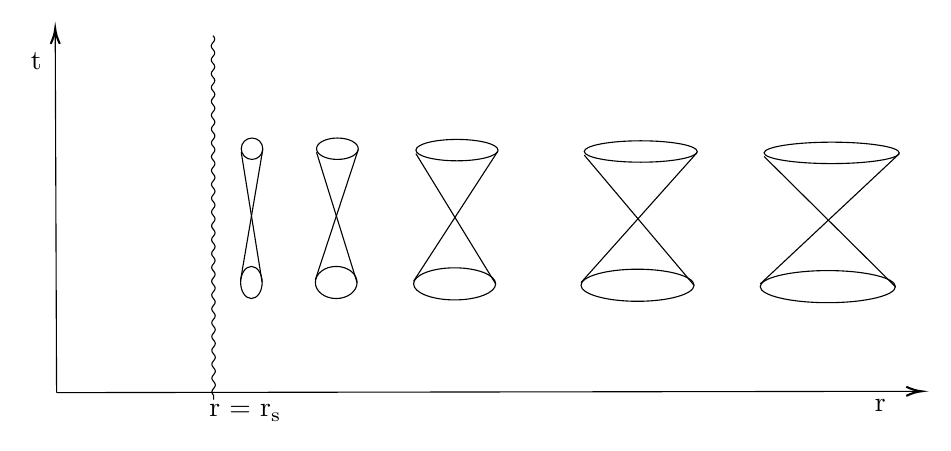
\begin{tikzpicture}[x=0.5pt,y=0.5pt,yscale=-1,xscale=1]

%Straight Lines [id:da6124197854166261] 
\draw    (30.49,272) -- (29.51,11) ;
\draw [shift={(29.5,9)}, rotate = 89.79] [color={rgb, 255:red, 0; green, 0; blue, 0 }  ][line width=0.75]    (10.93,-3.29) .. controls (6.95,-1.4) and (3.31,-0.3) .. (0,0) .. controls (3.31,0.3) and (6.95,1.4) .. (10.93,3.29)   ;
%Straight Lines [id:da9536673650889413] 
\draw    (30.49,272) -- (653.5,271.04) ;
\draw [shift={(655.5,271.03)}, rotate = 179.91] [color={rgb, 255:red, 0; green, 0; blue, 0 }  ][line width=0.75]    (10.93,-3.29) .. controls (6.95,-1.4) and (3.31,-0.3) .. (0,0) .. controls (3.31,0.3) and (6.95,1.4) .. (10.93,3.29)   ;
%Straight Lines [id:da48974690092852224] 
\draw    (143.5,14) .. controls (145.17,15.67) and (145.17,17.33) .. (143.51,19) .. controls (141.85,20.67) and (141.85,22.33) .. (143.52,24) .. controls (145.19,25.67) and (145.19,27.33) .. (143.53,29) .. controls (141.87,30.67) and (141.87,32.33) .. (143.54,34) .. controls (145.21,35.67) and (145.21,37.33) .. (143.55,39) .. controls (141.89,40.67) and (141.89,42.33) .. (143.56,44) .. controls (145.23,45.67) and (145.23,47.33) .. (143.57,49) .. controls (141.91,50.67) and (141.91,52.33) .. (143.58,54) .. controls (145.25,55.67) and (145.25,57.33) .. (143.59,59) .. controls (141.93,60.67) and (141.93,62.33) .. (143.6,64) .. controls (145.27,65.67) and (145.27,67.33) .. (143.6,69) .. controls (141.94,70.67) and (141.94,72.33) .. (143.61,74) .. controls (145.28,75.67) and (145.28,77.33) .. (143.62,79) .. controls (141.96,80.67) and (141.96,82.33) .. (143.63,84) .. controls (145.3,85.67) and (145.3,87.33) .. (143.64,89) .. controls (141.98,90.67) and (141.98,92.33) .. (143.65,94) .. controls (145.32,95.67) and (145.32,97.33) .. (143.66,99) .. controls (142,100.67) and (142,102.33) .. (143.67,104) .. controls (145.34,105.67) and (145.34,107.33) .. (143.68,109) .. controls (142.02,110.67) and (142.02,112.33) .. (143.69,114) .. controls (145.36,115.67) and (145.36,117.33) .. (143.7,119) .. controls (142.04,120.67) and (142.04,122.33) .. (143.71,124) .. controls (145.38,125.67) and (145.38,127.33) .. (143.72,129) .. controls (142.06,130.67) and (142.06,132.33) .. (143.73,134) .. controls (145.4,135.67) and (145.4,137.33) .. (143.74,139) .. controls (142.08,140.67) and (142.08,142.33) .. (143.75,144) .. controls (145.42,145.67) and (145.42,147.33) .. (143.76,149) .. controls (142.1,150.67) and (142.1,152.33) .. (143.77,154) .. controls (145.44,155.67) and (145.44,157.33) .. (143.78,159) .. controls (142.12,160.67) and (142.12,162.33) .. (143.79,164) .. controls (145.46,165.67) and (145.46,167.33) .. (143.79,169) .. controls (142.13,170.67) and (142.13,172.33) .. (143.8,174) .. controls (145.47,175.67) and (145.47,177.33) .. (143.81,179) .. controls (142.15,180.67) and (142.15,182.33) .. (143.82,184) .. controls (145.49,185.67) and (145.49,187.33) .. (143.83,189) .. controls (142.17,190.67) and (142.17,192.33) .. (143.84,194) .. controls (145.51,195.67) and (145.51,197.33) .. (143.85,199) .. controls (142.19,200.67) and (142.19,202.33) .. (143.86,204) .. controls (145.53,205.67) and (145.53,207.33) .. (143.87,209) .. controls (142.21,210.67) and (142.21,212.33) .. (143.88,214) .. controls (145.55,215.67) and (145.55,217.33) .. (143.89,219) .. controls (142.23,220.67) and (142.23,222.33) .. (143.9,224) .. controls (145.57,225.67) and (145.57,227.33) .. (143.91,229) .. controls (142.25,230.67) and (142.25,232.33) .. (143.92,234) .. controls (145.59,235.67) and (145.59,237.33) .. (143.93,239) .. controls (142.27,240.67) and (142.27,242.33) .. (143.94,244) .. controls (145.61,245.67) and (145.61,247.33) .. (143.95,249) .. controls (142.29,250.67) and (142.29,252.33) .. (143.96,254) .. controls (145.63,255.67) and (145.63,257.33) .. (143.97,259) .. controls (142.31,260.67) and (142.31,262.33) .. (143.98,264) .. controls (145.65,265.67) and (145.65,267.33) .. (143.98,269) .. controls (142.32,270.67) and (142.32,272.33) .. (143.99,274) -- (144,277) -- (144,277) ;
%Straight Lines [id:da08490630321795567] 
\draw    (541.79,101.31) -- (636.71,195.4) ;
%Straight Lines [id:da879557342815412] 
\draw    (639.5,99.38) -- (539,193.47) ;
%Shape: Ellipse [id:dp5886439559283081] 
\draw   (539,195.4) .. controls (539,188.99) and (560.87,183.8) .. (587.85,183.8) .. controls (614.84,183.8) and (636.71,188.99) .. (636.71,195.4) .. controls (636.71,201.81) and (614.84,207) .. (587.85,207) .. controls (560.87,207) and (539,201.81) .. (539,195.4) -- cycle ;
%Shape: Ellipse [id:dp7654739985131072] 
\draw   (541.79,98.73) .. controls (541.79,94.46) and (563.66,91) .. (590.65,91) .. controls (617.63,91) and (639.5,94.46) .. (639.5,98.73) .. controls (639.5,103) and (617.63,106.47) .. (590.65,106.47) .. controls (563.66,106.47) and (541.79,103) .. (541.79,98.73) -- cycle ;
%Straight Lines [id:da5733094312508271] 
\draw    (411.83,100.31) -- (491.17,194.4) ;
%Straight Lines [id:da643822488732185] 
\draw    (493.5,98.38) -- (409.5,192.47) ;
%Shape: Ellipse [id:dp023789317638629015] 
\draw   (409.5,194.4) .. controls (409.5,187.99) and (427.78,182.8) .. (450.33,182.8) .. controls (472.88,182.8) and (491.17,187.99) .. (491.17,194.4) .. controls (491.17,200.81) and (472.88,206) .. (450.33,206) .. controls (427.78,206) and (409.5,200.81) .. (409.5,194.4) -- cycle ;
%Shape: Ellipse [id:dp9347663056594007] 
\draw   (411.83,97.73) .. controls (411.83,93.46) and (430.12,90) .. (452.67,90) .. controls (475.22,90) and (493.5,93.46) .. (493.5,97.73) .. controls (493.5,102) and (475.22,105.47) .. (452.67,105.47) .. controls (430.12,105.47) and (411.83,102) .. (411.83,97.73) -- cycle ;
%Straight Lines [id:da5397882634375336] 
\draw    (290.19,99.31) -- (347.81,193.4) ;
%Straight Lines [id:da9061918081527438] 
\draw    (349.5,97.38) -- (288.5,191.47) ;
%Shape: Ellipse [id:dp01827528625348629] 
\draw   (288.5,193.4) .. controls (288.5,186.99) and (301.78,181.8) .. (318.15,181.8) .. controls (334.53,181.8) and (347.81,186.99) .. (347.81,193.4) .. controls (347.81,199.81) and (334.53,205) .. (318.15,205) .. controls (301.78,205) and (288.5,199.81) .. (288.5,193.4) -- cycle ;
%Shape: Ellipse [id:dp9530096373998713] 
\draw   (290.19,96.73) .. controls (290.19,92.46) and (303.47,89) .. (319.85,89) .. controls (336.22,89) and (349.5,92.46) .. (349.5,96.73) .. controls (349.5,101) and (336.22,104.47) .. (319.85,104.47) .. controls (303.47,104.47) and (290.19,101) .. (290.19,96.73) -- cycle ;
%Straight Lines [id:da5935431649480939] 
\draw    (218.36,98.31) -- (247.64,192.4) ;
%Straight Lines [id:da6313442873856193] 
\draw    (248.5,96.38) -- (217.5,190.47) ;
%Shape: Ellipse [id:dp3556374939552184] 
\draw   (217.5,192.4) .. controls (217.5,185.99) and (224.25,180.8) .. (232.57,180.8) .. controls (240.89,180.8) and (247.64,185.99) .. (247.64,192.4) .. controls (247.64,198.81) and (240.89,204) .. (232.57,204) .. controls (224.25,204) and (217.5,198.81) .. (217.5,192.4) -- cycle ;
%Shape: Ellipse [id:dp47694972976540695] 
\draw   (218.36,95.73) .. controls (218.36,91.46) and (225.11,88) .. (233.43,88) .. controls (241.75,88) and (248.5,91.46) .. (248.5,95.73) .. controls (248.5,100) and (241.75,103.47) .. (233.43,103.47) .. controls (225.11,103.47) and (218.36,100) .. (218.36,95.73) -- cycle ;
%Straight Lines [id:da5359111848439203] 
\draw    (163.94,98.31) -- (179.06,192.4) ;
%Straight Lines [id:da3296379646187486] 
\draw    (179.5,96.38) -- (163.5,190.47) ;
%Shape: Ellipse [id:dp397205529464427] 
\draw   (163.5,192.4) .. controls (163.5,185.99) and (166.98,180.8) .. (171.28,180.8) .. controls (175.57,180.8) and (179.06,185.99) .. (179.06,192.4) .. controls (179.06,198.81) and (175.57,204) .. (171.28,204) .. controls (166.98,204) and (163.5,198.81) .. (163.5,192.4) -- cycle ;
%Shape: Ellipse [id:dp70871059514235] 
\draw   (163.94,95.73) .. controls (163.94,91.46) and (167.43,88) .. (171.72,88) .. controls (176.02,88) and (179.5,91.46) .. (179.5,95.73) .. controls (179.5,100) and (176.02,103.47) .. (171.72,103.47) .. controls (167.43,103.47) and (163.94,100) .. (163.94,95.73) -- cycle ;

% Text Node
\draw (10,24) node [anchor=north west][inner sep=0.75pt]   [align=left] {t};
% Text Node
\draw (620,275) node [anchor=north west][inner sep=0.75pt]   [align=left] {r};
% Text Node
\draw (139,279) node [anchor=north west][inner sep=0.75pt]   [align=left] {r = r\textsubscript{s}};
\end{tikzpicture}
\bigskip


%%to add to diagram is the future of the cone and the past of the cone, add point to the center, add "P"
We see that the closer to the event horizon the steeper becomes the slope of the light-cone,















